\documentclass[11pt]{article}

\usepackage[T1]{fontenc}
\usepackage{geometry}
\usepackage{amsmath, amssymb, amsthm}
\usepackage[scr]{rsfso}
\usepackage[%
    hidealllines=true,%
    innerbottommargin=15,%
    nobreak=true,%
]{mdframed}
\usepackage{xcolor}
\usepackage{graphicx}
\usepackage{fancyhdr}
\usepackage{hyperref}

\geometry{a4paper, margin=1in, headheight=14pt}

\pagestyle{fancy}
\fancyhf{}
\renewcommand\headrulewidth{0.4pt}
\fancyhead[L]{\scshape MA3103}
\fancyhead[R]{\scshape \leftmark}
\rfoot{\footnotesize\it Updated on \today}
\cfoot{\thepage}

\newcommand{\C}{\mathbb{C}}
\newcommand{\R}{\mathbb{R}}
\newcommand{\Q}{\mathbb{Q}}
\newcommand{\Z}{\mathbb{Z}}
\newcommand{\N}{\mathbb{N}}

\newmdtheoremenv[%
    backgroundcolor=blue!10!white,%
]{theorem}{Theorem}[section]
\newmdtheoremenv[%
    backgroundcolor=violet!10!white,%
]{corollary}{Corollary}[theorem]
\newmdtheoremenv[%
    backgroundcolor=teal!10!white,%
]{lemma}[theorem]{Lemma}

\theoremstyle{definition}
\newmdtheoremenv[%
    backgroundcolor=green!10!white,%
]{definition}{Definition}[section]
\newmdtheoremenv[%
    backgroundcolor=red!10!white,%
]{exercise}{Exercise}[section]

\theoremstyle{remark}
\newtheorem*{remark}{Remark}
\newtheorem*{example}{Example}
\newtheorem*{solution}{Solution}

\surroundwithmdframed[%
    linecolor=black!20!white,%
    hidealllines=false,%
    innertopmargin=5,%
    innerbottommargin=10,%
    skipabove=0,%
    skipbelow=0,%
]{example}

\numberwithin{equation}{section}

\title{
    \Large\textsc{MA3103} \\
    \Huge \textbf{Introduction to Graph Theory and Combinatorics} \\
    \vspace{5pt}
    \Large{Autumn 2021}
}
\author{
    \large Satvik Saha
    \\\textsc{\small 19MS154}
}
\date{\normalsize
    \textit{Indian Institute of Science Education and Research, Kolkata, \\
    Mohanpur, West Bengal, 741246, India.} \\
}

\begin{document}
    \maketitle

    \tableofcontents

    \section{Introduction}
    
    \subsection{The Seven Bridges of K\"onigsberg}
    
    The diagram below depicts a region in the city of K\"onigsberg, Prussia. There
    are two islands, connected with the mainland and to each other via seven bridges.
    The Seven Bridges Problem is posed thus: is it possible to walk through the
    entire city, visiting each one of the four landmasses by crossing each of the
    bridges exactly once?

    \begin{center}
        \includegraphics[width=0.6\textwidth]{7_bridges.png}
    \end{center}

    Leonhard Euler showed that this is impossible; no such walk exists. The
    techniques he developed in doing so laid the foundations of \textit{graph
    theory}.

    The first thing to note is that the exact shape of the walk/trail is immaterial;
    all that matters is the sequence of landmasses visited and bridges crossed. Thus,
    each landmass can be compacted to a single point or \textit{vertex}, and each
    bridge a line or \textit{edge} connecting two such points. The resulting figure
    is a graph. Note that the orientations or placements of the points and lines are
    irrelevant, as long as the connections are undisturbed.

    \begin{center}
        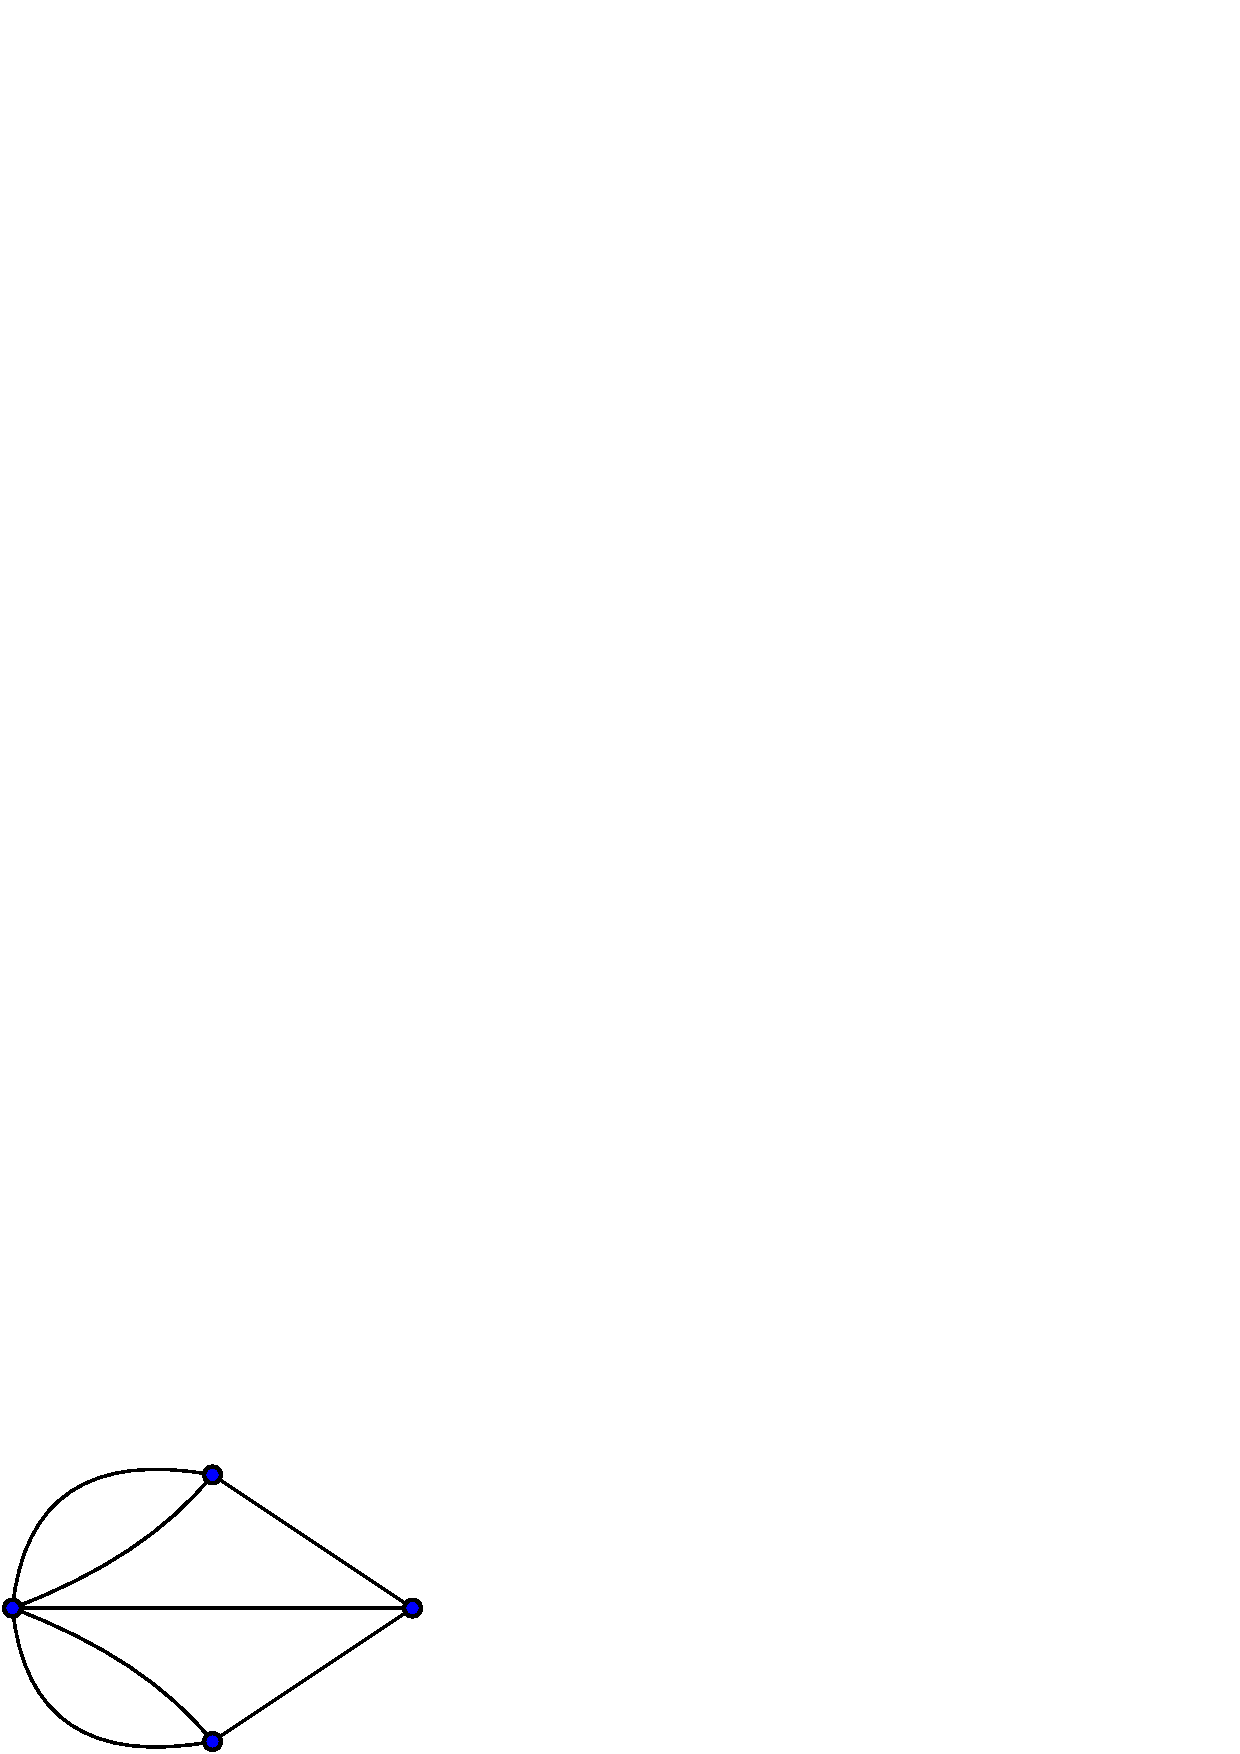
\includegraphics[width=0.5\textwidth]{7_bridges_graph.png}
    \end{center}

    Now, examine a landmass which is on the trail but is neither our starting point,
    nor our ending point. In order to reach this landmass, we must enter via a bridge; but
    we cannot stay in the landmass, so we must leave via another a bridge. Thus, for
    each time we pass through this landmass, we can cross off two bridges joined to
    it. Once we are done, no bridge may remain unused; this means that we must have
    started with an even number of bridges joined to this landmass.

    However, all four vertices in our graph connect to an odd number of edges. Since
    we require at least two vertices to act as intermediate points on our path, the
    desired walk is impossible.

\end{document}
